\subsection{The modelling principles}

\subsubsection{Definitions and notations}

The hypotheses and notations are presented in sections \ref{secDef} and \ref{secNot} respectively.

%{Basic modelling in the low flow channel of a reach}
\subsubsection{Basic modelling of a reach with low flow}

We use the well-established Saint-Venant equations :

\begin{itemize}
 \item the continuity equation :
   \begin{equation}
     \label{masse}
     \frac{\partial Q}{\partial x} + \frac{\partial S}{\partial t}= q_l
   \end{equation}
   with :
   \begin{itemize}
     \item $Q(x,t)$ the flow ($m^3.s^{-1}$);
     \item $Z(x,t)$ the elevation of the free surface ($m$).
   \end{itemize}

  \vspace{0.5cm}

 \item and the momentum equation :
   \begin{equation}
     \label{qmv}
     \frac{\partial Q}{\partial t} + \frac{\partial}{\partial x}\left( {\beta \frac{Q^2}{S}} \right) + g S \left( \frac{\partial Z}{\partial x} + J \right) = \gamma_l
   \end{equation}
   with $g$ the acceleration of gravity ($m.s^{-2}$).

\end{itemize}

\vspace{0.5cm}

The continuity equation relates to the conservation of the flow, the momentum equation corresponds to the fundamental equation of dynamics: the first member represents the accelleration of a \textit{volume of water}; the second member represents the sum of the forces applied to it.

\vspace{0.5cm}

When there is no lateral inflow : $q_l = \gamma_l = 0$. In the case of a lateral inflow, the version $7.1.4$ introduces two possible choices :

\begin{itemize}
 \item the inflow is considered perpendicular to the flow and does not bring any momentum : $\gamma_l = 0$
 \item the inflow modifies the momentum equation : $\gamma_l = \frac{Q}{S}q_l$
\end{itemize}

\vspace{0.5cm}

The term $gSJ$ relates to the effect of friction : $J$ is a dimensionless number, representing the average rate of the energy dissipation. It depends on the flow, the hydraulic characteristics of the river and of course, on the roughness coefficient. It is calculated with the Strickler relation:

   \begin{equation}
     J = \frac{Q^2}{K_{m}^{2}S^{2}R^{4/3}}
   \end{equation}
where
   \begin{equation}
     J = \frac{Q^2}{D^2}
   \end{equation}

with :
\begin{itemize}
 \item $K_m$ the Strickler's roughness coefficient;
 \item $R$ the hydraulic radius;
 \item $D$ the conveyance.
\end{itemize}

\vspace{0.5cm}

The dimensionless coefficient $\beta$ results from the variations of the actual flow velocity in a section. These variations would otherwise be ignored as only the average velocity is considered in the one-dimensional equations. The definition of $\beta$ is :

   \begin{equation}
     \beta = \frac{S}{Q^2} \int V^2 \,dS
   \end{equation}

\vspace{0.5cm}

Taking into account the hypotheses described previously (see section \ref{secDef}), in a single channel we consider: $\beta = 1$, i.e. we ignore the variations of velocity within a section. However, that is not the case for a compound channel. 

The boundary conditions in subcritical regime usually are: 
\begin{itemize}
 \item a discharge imposed at the upstream boundary;
 \item an elevation or, for unsteady flow a stage-discharge relationship, imposed at the downstream boundary.
\end{itemize}

\vspace{0.5cm}

In unsteady flow, it is possible (from a numeric point of view) to impose any types of boundary conditions (imposed elevation, discharge or a relationship between elevation and discharge) for both upstream and downstream boundaries. However, they have to be coherent to ensure that the algorithm runs successfully.



%{Modelling the compound channel of a reach}
\subsubsection{Modelling a reach with high flow: compound channel}

\paragraph{Problem to be solved\\}

\hspace*{1cm}

The problem that arises in this case is due to the fact that we cannot directly write a system of equations analog to (\ref{masse})(\ref{qmv}). The energy losses due to friction are not identical in the two parts of the compound channel, and therefore:
\begin{itemize}
 \item the hypothesis of a uniform velocity in a section and, in particular, a velocity identical in both the low flow and high flow channels, is not acceptable;
 \item we cannot define a priori a \textit{global} headloss coefficient $J$.
\end{itemize}

\vspace{0.5cm}


It is therefore necessary to write a system (\ref{masse})(\ref{qmv}) for the low flow channel (index $m$) and for the high flow channel (index $M$), which gives :

\begin{equation}
 \left \lbrace
  \begin{array}{l}
    \frac{\partial{S_m}}{\partial{t}} + \frac{\partial{Q_m}}{\partial{x}} = 0 \\
    \\
    \frac{\partial{Q_m}}{\partial{t}} + \frac{\partial}{\partial{x}} \left ( \frac{Q_{m}^2}{S_m} \right ) = -g S_m \frac{\partial{Z}}{\partial{x}} - g S_m J_m + \gamma_{mM}
  \end{array}
 \right.
\end{equation}

and

\begin{equation}
 \left \lbrace
  \begin{array}{l}
    \frac{\partial{S_M}}{\partial{t}} + \frac{\partial{Q_M}}{\partial{x}} = 0 \\
    \\
    \frac{\partial{Q_M}}{\partial{t}} + \frac{\partial}{\partial{x}} \left ( \frac{Q_{M}^2}{S_M} \right ) = -g S_M \frac{\partial{Z}}{\partial{x}} - g S_M J_M + \gamma_{Mm}
  \end{array}
 \right.
\end{equation}

with : $\gamma_{Mm} = -\gamma_{mM}$

\vspace{0.5cm}

With this formulation, we preserve the fundamental hypothesis: a free surface $Z$ identical in both the low flow channel and the high flow channel.

\vspace{0.5cm}

The term $\gamma_{mM}$ represents the interaction, initially unknown, between the two channels.
\vspace{0.5cm}

By adding the two systems, with the notation: $Q = Q_m + Q_M$ the total discharge, and : $S = S_m + S_M$ the total section, we can write:

\begin{equation}
 \label{sysGlob}
 \left \lbrace
  \begin{array}{l}
    \frac{\partial{S}}{\partial{t}} + \frac{\partial{Q}}{\partial{x}} = 0 \\
    \\
    \frac{\partial{Q}}{\partial{t}} + \frac{\partial}{\partial{x}} \left ( \frac{Q_{m}^2}{S_m} + \frac{Q_{M}^2}{S_M} \right ) = -g S \frac{\partial{Z}}{\partial{x}} - g ( S_m J_m + S_M J_M )
  \end{array}
 \right.
\end{equation}

with : $\sqrt{J_m} = \frac{Q_m}{D_m}$ et  $\sqrt{J_M} = \frac{Q_M}{D_M}$

\vspace{0.5cm}

The low flow and high flow conveyances depend on the free surface elevation $Z$ :

\begin{equation}
 \left \lbrace
  \begin{array}{l}
    D_m = K_m S_m R_{m}^{2/3} \\
    D_M = K_M S_M R_{M}^{2/3}
  \end{array}
 \right.
\end{equation}

\vspace{0.5cm}

The system (\ref{sysGlob}) is made similar to the system (\ref{masse})(\ref{qmv}) by defining a \textit{global} slope $J$ with the following relationship :

\begin{equation}
  SJ = S_m J_m + S_M J_M
\end{equation}

\vspace{0.5cm}

and by choosing a coefficient $\beta$, different from 1 but satisfying the relationship :

\begin{equation}
  \beta \frac{Q^2}{S} = \frac{Q_{m}^2}{S_m} + \frac{Q_{M}^2}{S_M}
\end{equation}

which gives:

\begin{equation}
  \beta =  \frac{S}{Q^2} \left ( \frac{Q_{m}^2}{S_m} + \frac{Q_{M}^2}{S_M} \right )
\end{equation}

\vspace{0.5cm}

We have now two additional unknowns, $Q_m$ and $Q_M$, so there are four unknowns in total with the two usual unknowns $Q$ and $Z$.

\vspace{0.5cm}

However we have the simple relationship:

\begin{equation}
  Q_m + Q_M = Q
\end{equation}

\vspace{0.5cm}

To solve the system (\ref{sysGlob}), it is necessary to write an additional differential equation or, more simply, to write an additional relationship linking the two unknowns. This relationship can be obtained by expressing the total conveyance $D$ according to the low flow and high flow conveyances $D_m$, $D_M$. First the slope $J$ is written as:

\begin{equation}
  S \frac{Q^2}{D^2} = S_m \frac{Q_{m}^2}{D_{m}^2} + S_M \frac{Q_{M}^2}{D_{M}^2}
\end{equation}

\vspace{0.5cm}

A simple assumption can be made, the slopes of the energy lines are identical in each channel :

\begin{equation}
  \frac{Q_m}{D_m} = \frac{Q_M}{D_M}
\end{equation}

\vspace{0.5cm}

Considering the definition of $J$, this is equivalent to set the global \linebreak conveyance as :

\begin{equation}
  D = D_m + D_M
\end{equation}

\vspace{0.5cm}

Due to its simplicity, this solution has the advantage of being easily generalised to a generic compound channel, i.e. comprised of more than two channels (low flow and high flow), each channel having a specific roughness. The considerations above remain valid, and it is sufficient to take the global conveyance as the sum of the conveyances of each channel.

\vspace{0.5cm}

However, this approach neglects the interactions between the channels, these interactions result in the energy lines being different. The following approach is developed to take into account this phenomenon.

\vspace{0.5cm}

First of all we define the generalised low flow and high flow conveyances $D_{mg}$, $D_{Mg}$ with the following relationships:

\begin{equation}
 \left \lbrace
  \begin{array}{l}
    Q_m =  D_{mg} \sqrt{J}\\
    Q_M =  D_{Mg} \sqrt{J}
  \end{array}
 \right.
\end{equation}

\vspace{0.5cm}

We consider the variable: $\eta = \frac{Q_m}{Q_M}$ and we use again the expression defining $J$, we can write:

\begin{equation}
    \frac{D_{mg}}{D_{Mg}} = \eta
\end{equation}

and also:

\begin{equation}
     D_{mg}^2 = \frac{S}{\displaystyle  \frac{S_m}{D_{m}^2}+ \frac{1}{\eta^2}\frac{S_M}{D_{M}^2}}
\end{equation}

\vspace{0.5cm}

We therefore establish that we only need to know the value of one of the following variables:$\eta$, $D_{mg}$, or $D_{Mg}$. Once one of these three variables is known, the others two can be calculated.

\vspace{0.5cm}

The system (\ref{sysGlob}) is therefore rewritten as:

\begin{equation}
 \label{sysFin}
 \left \lbrace
  \begin{array}{l}
    \frac{\partial{S}}{\partial{t}} + \frac{\partial{Q}}{\partial{x}} = 0 \\
    \\
    \frac{\partial{Q}}{\partial{t}} + \frac{\partial}{\partial{x}} \left ( \beta \frac{Q^2}{S} \right ) = -g S \frac{\partial{Z}}{\partial{x}} - g S J
  \end{array}
 \right.
\end{equation}

with :

\begin{equation}
 \left \lbrace
  \begin{array}{l}
    \beta = \left ( \frac{\eta^2}{S_m} + \frac{1}{S_M} \right ) \frac{S}{(1+\eta)^2} \\
    \\
    \sqrt{J} = \frac{Q}{D_{mg}+D_{Mg}}
  \end{array}
 \right.
\end{equation}

\vspace{0.5cm}

If either $\eta$, $D_{mg}$ or $D_{Mg}$ is known, the variables $\beta$ and $J$ are also known, and the system (\ref{sysFin}) is perfectly analog to the system (\ref{masse})(\ref{qmv}) established for a single channel. The solution gives the value of $Q$, and the following relationships provide the values of $Q_m$ and $Q_M$ :

\begin{equation}
  \eta = \frac{Q_m}{Q_M} = \frac{D_{mg}}{D_{Mg}}
\end{equation}

and :

\begin{equation}
  Q = Q_m + Q_M
\end{equation}

\vspace{0.5cm}

In this context, the \textit{simple} solution: $J_m = J_M = J$ (see above), is equivalent to:

\begin{equation}
  D_{mg} = D_m
\end{equation}

and : 

\begin{equation}
  D_{Mg} = D_M
\end{equation}

\paragraph{\emph{Debord} Modelling\\} \label{ModDeb}

\hspace*{1cm}

This approach allows to differentiate the roughness in the low flow channel and in the high flow channel.
It has been established experimentally, by studying the uniform regime
and by identifying a law of discharge distribution of the type: $\frac{Q_m}{Q_M}$ (see \cite{UAN75},\cite{NICOLLET79}).

\vspace{0.5cm}

The extrapolation to the gradually varied regime is appropriate, since this regime is defined as a succession of steady states.  

\vspace{0.5cm}

The approach is based on the following consideration: in a compound channel, under the conditions described above, the discharge in the low flow channel is equal to the discharge in an identical single channel multiplied by a characteristic value $A$ with : $A \in ]0,1[$.

\vspace{0.5cm}

$A$ is expressed as a function of the roughness of each bed. Its expression is given later, as the variables $D_{mg}$ and $D_{Mg}$ need to be calculated first.

\vspace{0.5cm}

With the assumption above we can writte: $D_{mg} = A D_m$, or : $Q_{m}^2 = A^2 D_{m}^2 J$.

\vspace{0.5cm}

We then derive $D_{Mg}$, by again using the expression of $J$:

\begin{equation}
  S J = S_m \frac{Q_{m}^2}{D_{m}^2} + S_M \frac{Q_{M}^2}{D_{M}^2} = A^2 S_m J + S_M \frac{Q_{M}^2}{D_{M}^2}
\end{equation}

This is equivalent to:

\begin{equation}
  J ( S - A^2 S_m ) = Q_{M}^2 \frac{S_M}{D_{M}^2}
\end{equation}

And we finally obtain:

\begin{equation}
  D_{Mg}^2 = \frac{Q_{M}^2}{J} = D_{M}^2 \left ( \frac{S - A^2 S_m}{S_M}  \right ) = D_{M}^2 \left ( 1 + \frac{S_m}{S_M} ( 1 - A^2 )  \right )
\end{equation}

\vspace{0.5cm}

The generalised high flow channel conveyance is therefore equal to the high flow channel conveyance multiplied by the value : 

$$
 \sqrt{1 + \frac{S_m}{S_M}(1-A^2)}
$$

\vspace{0.5cm}

When $A = 1$, we obtain the \textit{simple} model previously introduced. The ratio $\eta = \frac{Q_m}{Q_M}$ can be rewritten as:

\begin{equation}
  \eta = \frac{A}{\displaystyle \sqrt{1+\frac{S_m}{S_M}(1-A^2)}} \frac{D_m}{D_M}
\end{equation}

\vspace{0.5cm}

$A$ is the constant parameter of the \emph{Debord} model. It is evaluated with the relation:

\begin{equation}
  A = \frac{1-A_0}{2}\cos \left ( \frac{\pi r}{0.3} \right ) + \frac{1+A_0}{2} \quad \mbox{for} \quad r = \frac{R_M}{R_m} \in [0,0.3] 
\end{equation}

and :

\begin{equation}
  A = A_0 = 0.9 \left ( \frac{K_m}{K_M} \right )^{-1/6} \quad \mbox{for} \quad r > 0.3
\end{equation}

\vspace{0.5cm}

This equation has been derived from experiments on physical models.

\vspace{0.5cm}

It should be noted that $A$ varies with $R_m$ and $R_M$, so that $A = 1$ when $R_M = 0$ (no overflow).

\paragraph{\emph{Bottom-Bank} Modelling\\}

\hspace*{1cm}

This approach is introduced to deal with low flow channels where it is important to distinguish the roughness of the banks from the roughness of the bottom. We can however follow the method used in the previous paragraph: here the compound channel results from the association of the section above the bottom (in place of the low flow channel) and the section above the banks (in place of the high flow channel).

\vspace{0.5cm}

The theoretical framework is the Mulloffer-Einstein hypothesis \cite{NICOLLET79} for the composition of the roughness. This assumes that:
\begin{itemize}
 \item the slope of the energy lines are the same for the two flows;
 \item the velocities are also the same.
\end{itemize}

\vspace{0.5cm}

The first hypothesis leads to the simple method of the conveyances composition described in the previous paragraph. This would be enough to solve the problem as it has so far been described, but then the second hypothesis (equality of velocities) cannot be guaranteed to be true. To impose this, we have to consider that the wetted sections in each channel are also unknown, i.e. they are not derived from the free surface elevation. This is equivalent to considering that the limit between the flows is not given by the two verticals above the bottom on the right and left bank.

\vspace{0.5cm}

We use the index 1 for the \textit{bottom} flow and the index 2 for the \textit{banks} flow, and we introduce two additional unknowns $S_1$ and $S_2$. The two additional relationships are therefore :

\begin{itemize}
 \item the total surface : $S_1 + S_2 = S$;
 \item the equality of velocity : $\frac{Q_1}{S_1}=\frac{Q_2}{S_2}$ , which we aim to impose.
\end{itemize}

\vspace{0.5cm}

The total conveyance $D$ is calculated by introducing an equivalent roughness $k$ defined by :

\begin{equation}
  \label{rugEq}
  D = \frac{Q}{\sqrt{J}}= k S R^{2/3}
\end{equation}

\vspace{0.5cm}

The equality of the energy lines is accounted with the relationship:

\begin{equation}
  \label{EgLigCh}
  D = D_1 + D_2 = k_1 S_1 R_{1}^{2/3} + k_2 S_2 R_{2}^{2/3}
\end{equation}

and the equality of the velocities is accounted with the following relationship (\ref{EgVit}) where Strickler's friction relation is applied to each flow section:

\begin{equation}
  \label{EgVit}
  k_1 R_{1}^{2/3} = k_2 R_{2}^{2/3}
\end{equation}

\vspace{0.5cm}


By combining the relationships (\ref{rugEq})(\ref{EgLigCh})(\ref{EgVit}) we immediately obtain :

\begin{equation}
  k R^{2/3} = k_1 R_{1}^{2/3} = k_2 R_{2}^{2/3}
\end{equation}

\begin{equation}
  R_1 = \frac{S_1}{P_1}
\end{equation}

\begin{equation}
  R_2 = \frac{S_2}{P_2}
\end{equation}

\begin{equation}
  R = \frac{S}{P}
\end{equation}

\vspace{0.5cm}

from which we can deduce the expression of $k$ characterising the composition of roughness :

\begin{equation}
  k^{3/2} = \frac{P}{\displaystyle \frac{P_1}{k_{1}^{3/2}}+\frac{P_2}{k_{2}^{3/2}}}
\end{equation}

\vspace{0.5cm}

Eventually, this approach is equivalent to considering a single bed whose roughness is the function of water depth, and is given by the formula above.

\subsubsection{Treatment of the storage zones}

The storage zones\footnote{Note that these are part of the cross-sections. Storage areas can also be described with storage cells. This modelling approach is described in section \ref{SectionCASIER}} 
act on the flow by abstracting or returning some water, but this water is not included in the energy balance. Consequently, in the continuity equation the wetted section is the total section (including the storage area), while in the dynamic equation the wetted section is only the area of the active bed (low flow and high flow only). In the flow equations, the wetted section often intervenes through its derivative with respect to the elevation i.e. the surface width $L$. Similarly, it is therefore the total surface width or the active bed width that must be used, depending on the equation considered. 
Storage areas are ignored in steady flow simulations.

\vspace{0.5cm}

The continuity equation can therefore be written as:

\begin{equation}
  \frac{\partial{(S + S_s)}}{\partial t} + \frac{\partial Q}{\partial x} = q_l
\end{equation}

which is equivalent to:

\begin{equation}
  (L + L_s) \frac{\partial Z}{\partial t} + \frac{\partial Q}{\partial x} = q_l
\end{equation}

and we finally have:

\begin{equation}
  L \frac{\partial Z}{\partial t} + \frac{\partial Q}{\partial x} = q_l - L_s \frac{\partial Z}{\partial t} = q_l + q_s
\end{equation}

the index $s$ indicating the variables relating to storage.

\vspace{0.5cm}

The storage is therefore equivalent to introducing a lateral discharge $q_s$ (assumed perpendicular). The influence of the sinuosity of the bed could be accounted by introducing an additional parameter $s$ in the following form :

\begin{equation}
  q_l = - s L_s \frac{\partial Z}{\partial t}
\end{equation}

\vspace{0.5cm}

However this is not done because of the difficulty of accurately evaluating $L_s$.
%JLH comment: is it not 'evaluating $s$' !?!?!

\vspace{0.5cm}

It is recalled that the water surface elevation used for the storage zones is identical to that used in the low and high flow channels, unlike with the storage cells (see section \ref{SectionCASIER}).



\subsubsection{Treatment of inflows}
\label{TraitAp}

We consider a lateral inflow $q_l$, expressed in $m^2.s^{-1}$ (discharge per unit length).

\vspace{0.5cm}

The flow equations are obtained from the system (\ref{masse})(\ref{qmv}) by adding $q_l$ to the second member of the continuity equation, and $k q_l V_l$ to the second member of the dynamic equation (indicating respectively the contribution of mass and momentum).

\vspace{0.5cm}

The coefficient $k$ results from the fact that the contribution of momentum depends on the respective axes of the main flow and the inflow; only the velocity in the direction of the main flow needs to be taken into account. Therefore, $k$ is nil for an inflow perpendicular to the axis of the main flow, 
and $k$ is theoretically equal to 1 for an inflow with the same direction as the main flow.

\vspace{0.5cm}

The standard version of \texttt{MASCARET} imposes $k = 0$, this deals with the most useful case and avoids the user to enter an additional parameter.

\vspace{0.5cm}

This modelling of inflows is therefore indicated for cases of \textit{diffuse} inflows where the inflow momentum is usually negligible compared to that of the main flow. In other cases it is preferable to explicitly create a reach representing the inflow (branched network), which would be equivalent to have $k = 1$.



\subsubsection{Treatment of junctions}
\label{TrNd}

The equations of Saint-Venant apply only between two sections of the same reach (see also the treatment of the singularities \ref{TS}). At each junction or node in a network, it is necessary to use alternative equations. 
These are derived from the equality of the elevations and the conservation of the discharges at the junction. 
The method is described below (see figure \ref{SchemConf}) on a simple example (no head losses considered), but can be generalised to a more complex situation.

\begin{figure}
 \begin{center}
  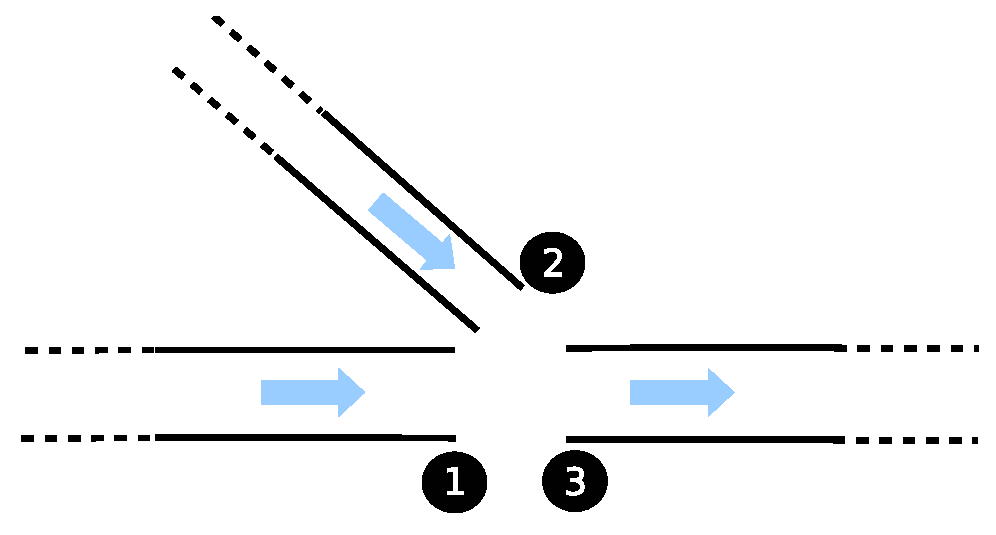
\includegraphics[scale=0.5]{Figures/Schema_confluent.eps}
  \caption{Diagram of a confluence with 3 reaches}
  \label{SchemConf}
 \end{center}
\end{figure}

\vspace{0.5cm}

The junction is bounded by three sections (numbered 1, 2 and 3) located at each end of the associated reaches. These sections are characterized by the hydraulic variables $(Q_1,Z_1)$, $(Q_2,Z_2)$ et $(Q_3,Z_3)$.

\vspace{0.5cm}

We can establish the equations used at the junction by considering the following simple case :
\begin{itemize}
 \item single channel;
 \item steady flow;
 \item velocities along the axis of each branch are identical in the 3 considered sections
% wetted sections such that the velocities along the average axis of the confluence are identical in each branch;
 \item no friction in the junction
 %no friction along the confluent. 
\end{itemize}

\vspace{0.5cm}

We can write the Saint-Venant equations along the reach defined by section no. 1 and section no. 3 (the reach corresponding to section no. 2 being treated as lateral contribution - see the previous section \ref{TraitAp})

%axis of the confluent by considering section no. 1 and then section no. 3 .

\vspace{0.5cm}

The continuity equation immediately gives:

\begin{equation}
  Q_3 - Q_1 = Q_2
\end{equation}

\vspace{0.5cm}

The dynamic equation becomes:

\begin{equation}
  V \frac{\partial Q}{\partial x} + g S \frac{\partial}{\partial x} \left ( Z + \beta \frac{V^2}{2 g} \right ) = k q_l V_l
\end{equation}

\vspace{0.5cm}

where $k$ is the coefficient of momentum as indicated in section \ref{TraitAp}.

\vspace{0.5cm}

The key hypothesis is the conservation of velocities along the axis. It means that:

\begin{equation}
  V = k V_l
\end{equation}

and:

\begin{equation}
  \frac{\partial}{\partial x} \left ( \beta \frac{V^2}{2g} \right ) = 0
\end{equation}

We can also write:

\begin{equation}
  \frac{\partial Q}{\partial x} = q_l
\end{equation}

\vspace{0.5cm}

The dynamic equation can therefore be reduced to:

\begin{equation}
  \frac{\partial Z}{\partial x} = 0
\end{equation}

which is equivalent to:

\begin{equation}
  Z_3 = Z_1
\end{equation}

\vspace{0.5cm}

Using a similar reasoning, we consider now the reach defined by sections no. 2 and no. 3, the reach of section no. 1 being treated as inflow, therefore we obtain : $Z_3 = Z_2$.

\vspace{0.5cm}

In summary, the continuity equation gives the conservation of discharges at the junction, and the dynamic equation gives the equality of the water levels.

\vspace{0.5cm}

In a general case, the simple hypotheses used previously are not verified, in particular:
\begin{itemize}
 \item the velocities in each branch are rarely similar;
 \item although friction can often be neglected, singular head losses need to be considered (see the following section).
\end{itemize}

\vspace{0.5cm}

However, the simple relationships obtained here are applied in the subcritical engines. They are the only equations that can be easily implemented in an algorithm.

\vspace{0.5cm}

In practice, the conservation of discharges is always respected, however, the equality of water levels poses a problem. To overcome this difficulty it is usually better to:
\begin{itemize}
 \item place the sections 1-2-3 as close as possible to the junction (to create a \textit{point} junction);
 %choose the closest possible extreme sections (\textit{punctual} confluence);
 \item introduce singular head losses on the branches upstream of the junction to account for the additional dissipation of energy (see the report on confluents in the bibliography and the following section).
\end{itemize}

\subsubsection{Singular head losses}

In the dynamic equation, the term $J$ represents the head losses known as linear, which result from the friction on the bottom and the banks. Localised head losses, known as singular head losses, can be produced in the presence of obstacles, rapid variations of sections or junctions. 
They are modeled by the mean of a term $J_s$, in addition to $J$ :
\begin{itemize}
 \item for a widening : $J_s = \xi_1 \frac{1}{2 g}(\beta_j V_j - \beta_i V_i)^2$ with :
   \begin{itemize}
     \item the indexes $j$ and $i$ denote respectively the upstream section and the downstream section;
     \item with: $\beta_j V_j < \beta_i V_i$.
   \end{itemize}
 \item for an obstacle placed immediately downstream of the section $j$ : \\ $J_s = \xi_2 \frac{1}{2g} \beta_j V_{j}^2$.
\end{itemize}
\vspace{0.5cm}
where $\xi_1$ and $\xi_2$ are the head losses coefficients.

\vspace{0.5cm}

In the current version of \texttt{MASCARET}, the value of $\xi_1$ is a fixed constant equal to 0.3 (based on the litterature), this is valid for gradual widenings (these are automatically taken into account).

\vspace{0.5cm}

The value of $\xi_2$ is set by the user and would often be chosen via a calibration. 
A singular head loss modelled with $\xi_2$ needs to be introduced whenever the head loss does not result from a progressive widening 
\footnote{This head loss is to be placed at the section $i = j + 1$ : in subcritical flow, with the downstream influencing the upstream, a head loss placed at the section $i$ will increase the head calculated at the section $j = i - 1$, and not reduce the head calculated at the section $i$.} 
(sudden narrowing or widening like bridges, etc.).



\subsubsection{Singularities} \label{singu}

\paragraph{General principle\\}

\hspace*{1cm}

The most common singularities are weirs or control dams. However, we will treat this problem more generally by refering to a singularity for any section of the river where the equations of Saint-Venant cannot be applied.

\vspace{0.5cm}

Therefore, in place of the Saint-Venant equations, it is necessary to use specific equations (transfer relationships) that define the influence of the singularity in order to carryout the water line calculations.

\vspace{0.5cm}

We assume that the singularity is located between two computational sections of indices $i$ and $j$ with : $i = j + 1$ (see figure \ref{SchemSing}).

\begin{figure}
 \begin{center}
  \includegraphics[scale=0.8,angle=270]{Figures/Schema_singularite.eps}
  \vspace{0.5cm}
  \caption{Diagram of a singularity}
  \label{SchemSing}
 \end{center}
\end{figure}

\vspace{0.5cm}

The continuity equation is reduced to $Q_i = Q_j$, expressing the equality of discharge on each side of the singularity. In unsteady flow, this introduces a slight discrepancy, the volume of water being no longer rigorously conserved. However, this bias is negligible if the distance separating the two calculation sections is \textit{reasonably small}.

\vspace{0.5cm}

The dynamic equation is specific to each type of singularity. Its general expression is : $f(Q, Z_{us},Z_{ds}) = 0$. 
The function $f$ is only used in its discretised form in the solution algorithm (see section \ref{MR}).
The equations used for each type of singularity are indicated in the following sections. A summary of the different singularities available in \texttt{MASCARET} is shown in section \ref{BilanSing}.

\paragraph{Weirs\\}

\hspace*{1cm}

In the most general form, the equation for weirs (see the figures hereafter) is of the form : $Q = f(Z_{us},Z_{ds})$, the type of flow (drowned or free flow) is directly integrated in the expression of the function $f$. 
$f$ is given in a discretised form with a sufficient series of triplets $(Q,Z_{us},Z_{ds})$.

\begin{itemize}
 \item \textsf{Free flow weir} : the discharge  $Q_d$ depends only on the upstream water level (see figure \ref{Sd});
   \begin{figure}
     \begin{center}
        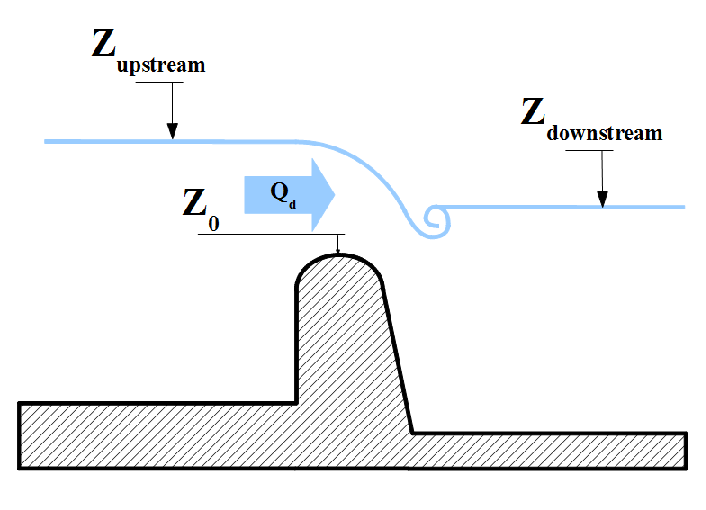
\includegraphics[scale=1.]{Figures/Schema_Seuil_Denoye.eps}
        \caption{Free flow weir }
        \label{Sd}
     \end{center}
    \end{figure}
   \\
   with $Q = Q_d = m L \sqrt{2g} (Z_{us}-Z_0)^{3/2}$ and :
      \begin{itemize}
        \item $m$ : the discharge coefficient;
        \item $L$ : the width of the weir. 
      \end{itemize}

 \item \textsf{Drowned weir}  ; the discharge $Q_n$ is influenced by the downstream water level (see figure \ref{Sn});
    \begin{figure}
     \begin{center}
        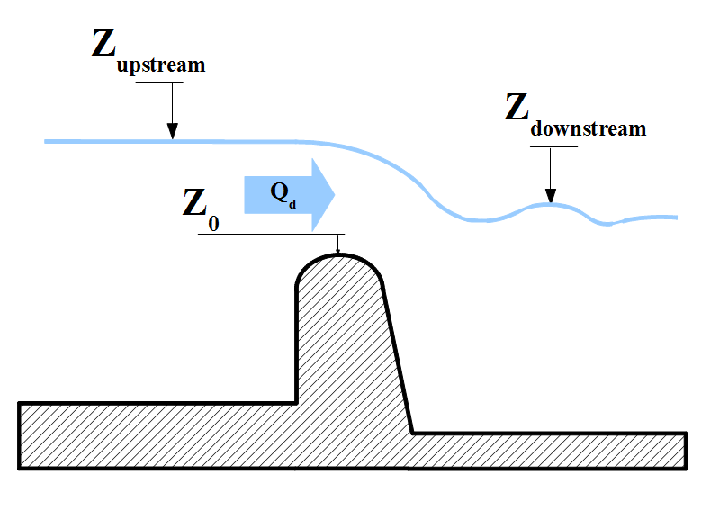
\includegraphics[scale=1.]{Figures/Schema_Seuil_Noye.eps}
        \caption{Drowned Weir}
        \label{Sn}
     \end{center}
    \end{figure}
    \\
    with $Q = Q_n = C Q_d$ and :
    \begin{itemize}
      \item $C$ : the drowned/free flow coefficient : $C = k \frac{Z_{ds}-Z_{0}}{Z_{us}-Z_0}$;
      \item $k$ : a function to be defined.
    \end{itemize}

\end{itemize}

\vspace{0.5cm}

The discharge law for the weir can also be defined only for free flow conditions (the downstream level does not influence the upstream level), in the form : $Q = f(Z_{us})$, i.e. by indicating a series of pairs $(Q,Z_{us})$.

\vspace{0.5cm}

The flow regime is considered as drowned when : $R = \frac{Z_{ds}-Z_0}{Z_{us}-Z_0}$ is greater than a threshold value $R_0$ (the crest elevation $Z_0$ is a parameter of the weir). An automatic correction is therefore applied : $Q = k(R) f(Z_{us})$. In \texttt{MASCARET} the value of the constant $R_0$, and the form of the function $k$, are imposed.

\vspace{0.5cm}

In the current version of \texttt{MASCARET}, two types of drowned weirs are distinguished with one relation for sharp-crested weirs and another one for broad-crested weirs (see section \ref{LoiSeuilMinceEpais}). For a broad-crested weir, $Ro$ is equal to 0.8, and $k$ is a parabolic function defined by :

\begin{equation}
  k(R) = -25 R^2 + 40 R -15
\end{equation}
with :
\begin{itemize}
 \item $k(R_0) = 1$;
 \item and $k(1) = 0$.
\end{itemize}

\vspace{0.5cm}

The weir can also be defined by the geometry of the crest, in this case the relation applied for free flow is a spill equation :


\begin{equation}
  Q = m \sqrt{2 g} \sum_{k} L_k (Z_{us} - Z_k)^{3/2}
\end{equation}

where :
\begin{itemize}
 \item $L_k$ is the length of an element of the crest with an elevation $Z_k$;
 \item $m$ is the discharge coefficient (a parameter of the weir).
\end{itemize}

\vspace{0.5cm}

In drowned flow, the discharge correction is identical to that defined above for a broad-crested weir.



\paragraph{Control Structures\\}

\hspace*{1cm}

The equation for the singularity is simply the imposed upstream water level (varying with time).



\paragraph{Control Sections\\}

\hspace*{1cm}

The equation for the singularity is a generic relation of the type : $Q = f(Z_{us})$.

\vspace{0.5cm}

A relation : $Q = f(Z_{ds})$ can also be specified but it exists only to enable some specific tests because it does not make physical sense in a subcritical flow regime. 


\subsubsection{Surcharged flow}

Sections where the flow is surcharged (e.g. under a bridge) do not require a specific treatment in the code. 
This is because the cross-sections incorporate a vertical slot with negligible width (the Preissmann slot) at the top of the section. When the cross-section is surcharged, the calculated water level $Z$ is higher than the soffit (top) level of the section, and the pressure $P$ is calculated by means of the relationship : $P = \rho g Z$ .

%These sections are taken into account in the geometry of the profiles. The sections under load must be topped by a vertical slot with negligible width (the Preissmann slot). If the section is indeed under load, the calculated elevation $Z$ will be greater than the obvert level of the section, and will give a value of pressure $P$ by means of the relationship : $P = \rho g Z$ .

